\documentclass{slides}
\title{Main Opmode Flow}
\author{Natan Jurca}
\date{September 2025}

\usepackage{tikz}
\usetikzlibrary{shapes.geometric, arrows}
\usetikzlibrary{positioning}

\tikzstyle{startstop} = [rectangle, rounded corners, minimum width=3cm, minimum height=1cm,text centered, draw=black, fill=red!30]
\tikzstyle{io} = [trapezium, trapezium left angle=70, trapezium right angle=110, minimum width=3cm, minimum height=1cm, text centered, draw=black]
\tikzstyle{process} = [rectangle, minimum width=3cm, minimum height=1cm, text centered, draw=black]
\tikzstyle{decision} = [diamond, aspect=2, minimum width=3cm, minimum height=1cm, text centered, draw=black]
\tikzstyle{arrow} = [thick,->,>=latex]

\begin{document}
\resizebox{!}{\textheight}{%
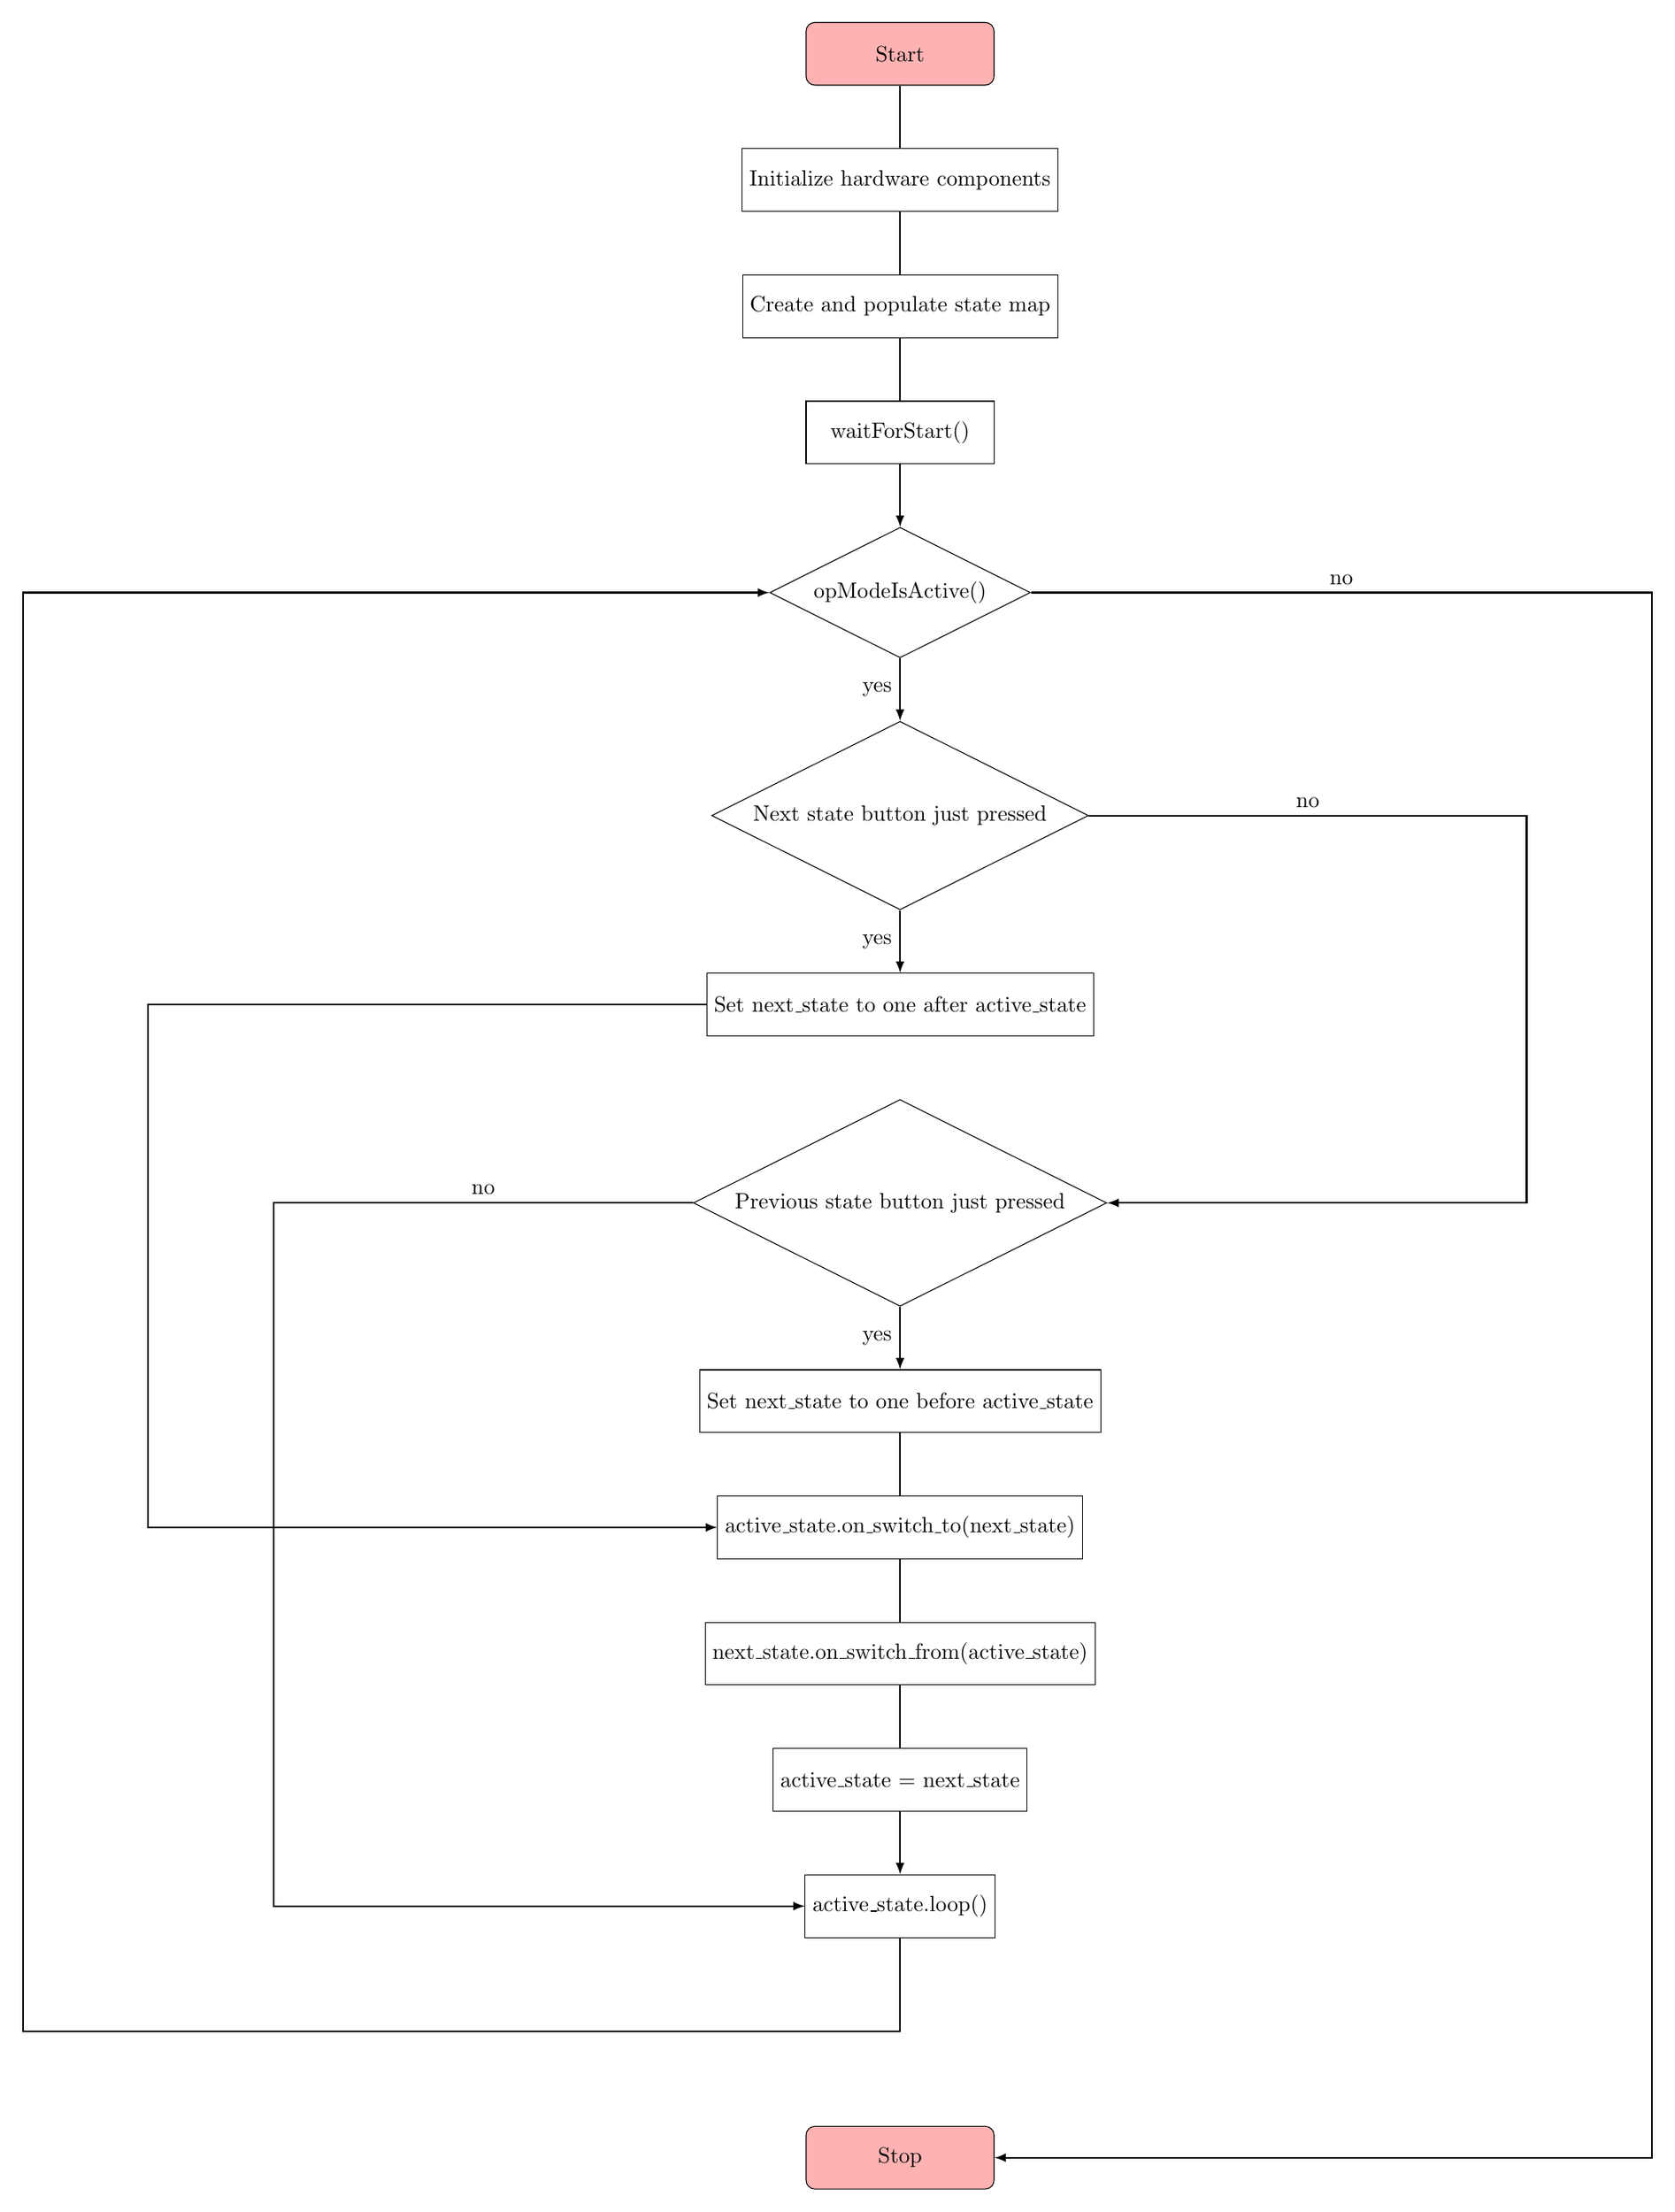
\begin{tikzpicture}[node distance=1cm]
	\node (start) [startstop] {Start};
	\node (create_init_hardware) [process, below=of start] {Initialize hardware components};
	\node (populate_state_map) [process, below=of create_init_hardware] {Create and populate state map};
	\node (wait_for_start) [process, below=of populate_state_map] {waitForStart()};
	\node (while_opmode_running) [decision, below=of wait_for_start] {opModeIsActive()};
	\node (is_next_state_just_pressed) [decision, below=of while_opmode_running] {Next state button just pressed};
	\node (determine_next_state) [process, below=of is_next_state_just_pressed] {Set next\_state to one after active\_state};
	\node (is_previous_state_just_pressed) [decision, below=of determine_next_state] {Previous state button just pressed};
	\node (determine_next_state_prev) [process, below=of is_previous_state_just_pressed] {Set next\_state to one before active\_state};
	\node (current_on_switch_to) [process, below=of determine_next_state_prev] {active\_state.on\_switch\_to(next\_state)};
	\node (next_on_switch_from) [process, below=of current_on_switch_to] {next\_state.on\_switch\_from(active\_state)};
	\node (set_next_active) [process, below=of next_on_switch_from] {active\_state = next\_state};
	\node (current_state_loop) [process, below=of set_next_active] {active\_state.loop()};
	\node (stop) [startstop, below=of current_state_loop, yshift=-2.0cm] {Stop};

	\draw [arrow] (start) -> (create_init_hardware) -> (populate_state_map) -> (wait_for_start) -> (while_opmode_running);

	\draw [arrow] (while_opmode_running) -> node[anchor=east] {yes} (is_next_state_just_pressed);
	\draw [arrow] (while_opmode_running) -- node[anchor=south] {no} ++(12cm, 0) |- (stop);

	\draw [arrow] (is_next_state_just_pressed) -> node[anchor=east] {yes} (determine_next_state);
	\draw [arrow] (is_next_state_just_pressed) -- node[anchor=south] {no} ++(10cm, 0) |- (is_previous_state_just_pressed);

	\draw [arrow] (determine_next_state) -- ++(-12cm, 0) {} |- (current_on_switch_to);

	\draw [arrow] (is_previous_state_just_pressed) -> node[anchor=east] {yes} (determine_next_state_prev);
	\draw [arrow] (is_previous_state_just_pressed) -- node[anchor=south] {no} ++(-10cm, 0) |- (current_state_loop);

	\draw [arrow] (determine_next_state_prev) -> (current_on_switch_to) -> (next_on_switch_from) -> (set_next_active) -> (current_state_loop);

	\draw [arrow] (current_state_loop) |- ++(-14.0cm, -2.0cm) {} |- (while_opmode_running);

\end{tikzpicture}%
}
\end{document}
